\subsection{Specific Aim 3: Self-assembly of Janus particles in ionic solutions}
\label{subsec:specific_aim_3}

\subsubsection{Dynamics of a single Janus particle in ionic solutions}
In experiments, Janus particles are often immersed in a solution of ions \cite{ChenWhitmer2011_Sci} or surfactants \cite{}.
In electrolytic solutions the interaction between salt and Janus particle gives 
rise to a slip velocity (on the particle surface) that depends on the ion distribution and the zeta potential \cite{BayatiJCP2016} 
(the potential difference between the Janus particle surface and the surrounding conducting fluid).
The short-range interactions between Janus particles depend on the salt concentration:
At very low salt concentrations, Janus particles repel one another electrostatically, whereas at high salt concentration, van der Waals
forces cause Janus particles to aggregate irreversibly \cite{Goodwin2019}. At intermediate concentrations of monovalent salt, Janus particles are found to self assemble in the form of a small number of elemental units of building blocks \cite{Chen2011_Science}. 
%
\begin{wrapfigure}[11]{l}{0.47\textwidth}
\centerline{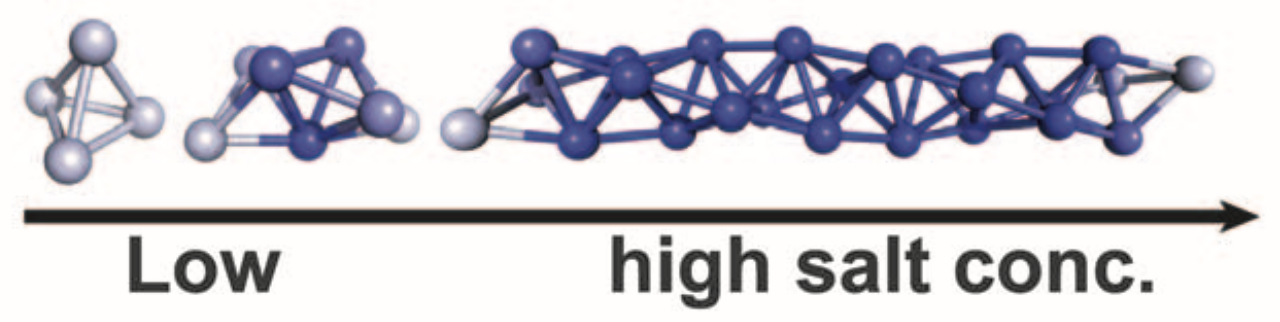
\includegraphics[width=0.46\textwidth]{Figures/fig2A_Chen2011_Science}}
  \vspace{-5pt}
\caption{\label{fig:helices_of_JPs} \footnotesize Formation of helices of Janus particles as salt concentration increases \cite{Chen2011_Science}.}
\end{wrapfigure}
%
Figure~\ref{fig:helices_of_JPs} shows that Janus particles can self-assemble into a helix at high concentration of monovalent salt (NaCl) when the density of Janus particles is low to moderate. At high density, JPs are found to form wormlike structures

The Stokes equations in~\eqref{eq:stokes} are modified to incorporate the transport of ions as
\begin{equation}
\label{eq:stokes}
\begin{aligned}
  &-\mu \Delta \mathbf{u} + \nabla p = \Delta\psi\cdot\nabla\psi, \quad \mathbf{x} \in \Omega, \qquad
  \nabla \cdot \mathbf{u} = 0,  \quad \mathbf{x} \in \Omega,\\
  &\delta^2\Delta\psi = -\frac{1}{2}\left(n_+-n_-\right),\qquad
  \frac{\partial n_{\pm}}{\partial t} + \nabla\cdot{\bf j}_{\pm} = 0,\\
  &{\bf j}_{\pm} = -\nabla n_{\pm} \mp n_{\pm} \nabla\psi + Pe n_{\pm}\mathbf{u}.
\end{aligned}
\end{equation}
The screen length $\rho$ is now a function of the ion concentrations: $\rho = \rho(n_+,n_-)$. 






\subsubsection{Electromechanical effects on the dynamic assembly of amphiphiles \label{subsubsec:em_effects}}
In recent experiments~\cite{FaizEtAl2019_SoftMatt}, membrane bending
rigidity was determined as a function of lipid composition from 0 to 100
mol $\%$ of charged lipids using flicker spectroscopy of the shape
fluctuations of a giant unilamellar vesicle (GUV).
%the bending rigidity is determined as a
%function of lipid composition from 0 to 100 mol $\%$ of charged lipids
%in recent experiments~\cite{FaizEtAl2019_SoftMatt}---
Membrane bending rigidity increases with increasing lipid surface
charge, but decreases with increasing salt concentration in the bulk
solution due to the screening of the lipid surface charge. This
result agrees
with several theoretical models~\cite{Kralchevsky1996_JCIS,
May1996_JChemPhys, LoubetEtAl2013_PRE} that also assume the quadratic
form of the elastic energy density in the presence of surface charge and
bulk charge~\cite{DuplantierGoldstein1990_PRL, Winterhalter1992_JPC}. As
the electrostatic interaction is non-local in nature, we expect that the
controversy of the HK elastic energy form (see
\S\ref{subsec:specific_aim_1}) would worsen in the presence of
electrostatic interactions and electrokinetics. The PIs will extend the
approaches in \S\ref{subsec:specific_aim_1} to charged lipids to
calculate the bending moduli and compare against the experimental
results in~\cite{FaizEtAl2019_SoftMatt}. We propose to incorporate an
explicit surface charge on each particle boundary $P_i$ and compute the
electrostatic potential as a functional of particle configuration.
Adding the electrostatic force to the hydrophobic attraction force
between particles, we will assess the dependence of elastic moduli on
electric charges using the methods described in
\S\ref{subsec:specific_aim_1}. Results from these proposed calculations
will provide further comparisons and validations of the HAP model
against the continuum mechanics.

Once the effects of lipid charges on the moduli are verified, the PIs
propose to examine how to use an external electric field to control the
amphiphilic self-assembly in solvent. PI YNY has a track record of
working on electrohydrodynamics of an elastic, inextensible membrane
using both asymptotic analysis~\cite{Nganguia2013_PRE, Young2014_JFM,
Young2015_PoF} and numerical simulations~\cite{Nganguia2015_CiCP} and
will work with both PIs RR and BQ to extend the HAP model to study the
electromechanical effects on the assembly of amphiphile. Results from
this research will yield a quantitative understanding of how to utilize
an electric field to achieve optimal control of assembly of amphiphiles
in solvent.




